% !TeX spellcheck = en_US
\documentclass[ twoside,openright,titlepage,numbers=noenddot,headinclude,%1headlines,% letterpaper a4paper
footinclude=true,cleardoublepage=empty,abstractoff, % <--- obsolete, remove (todo)
BCOR=10mm,paper=a4,fontsize=11pt,%11pt,a4paper,%
ngerman,american]{scrreprt} %,pdftex, xcolor=dvipsnames
\usepackage{acronym} %printonlyused,withpage
\usepackage{amsmath,amssymb}
\usepackage[ngerman,american]{babel}
%\usepackage[utf8]{inputenc}
%\usepackage[T1]{fontenc}         
\usepackage[hypertexnames=false]{hyperref}
\usepackage[parts]{classicthesis} % ,manychapters, dottedtoc, drafting
\usepackage{colortbl}
%
\usepackage{tikz}
\usetikzlibrary{shapes,snakes}
\usepackage{verbatim}
\tikzstyle{mybox} = [draw=red, fill=blue!20, very thick,
rectangle, rounded corners, inner sep=10pt, inner ysep=20pt]
\tikzstyle{fancytitle} =[fill=red, text=white]
%
\usepackage[final]{pdfpages}
\usepackage[titles]{tocloft}
\hypersetup{linktocpage=true,bookmarksnumbered=true,pageanchor=true,hypertexnames=false,naturalnames=true,plainpages=false}
\usepackage{tabto} % for tabbing
\usepackage{capt-of}
\usepackage{multicol} 
\usepackage{dcolumn}
\usepackage{supertabular}
\usepackage{tabularx}
\usepackage{upgreek}
\usepackage{enumitem}
\usepackage{doi}
\usepackage[style=authoryear-comp,natbib=true,backend=biber,uniquename=false,sortcites=false,maxnames=2,maxbibnames=99]{biblatex}
%\usepackage{framed, color}
%\definecolor{shadecolor}{rgb}{1.0, 0.72, 0.77}

\addtolength{\footskip}{5mm}
\addtolength{\oddsidemargin}{-1cm}
\addtolength{\evensidemargin}{-1cm}
\addtolength{\textwidth}{2cm}

\renewcommand{\cftchappresnum}{\scshape\MakeTextLowercase}%
\renewcommand{\cftchapfont}{\color{Maroon}\roman{part}\small\textsc}%textbf}%

\usepackage[format=hang]{caption}[2008/08/24]
\usepackage{textcomp}
\usepackage{todonotes}
\usepackage{fontawesome}
\usepackage{rotating}
\usepackage{pdflscape}
\usepackage{longtable}
\usepackage{afterpage}
\usepackage{physics}

\usepackage[separate-uncertainty=true, quotient-mode=fraction]{siunitx}
\DeclareSIUnit{\AU}{AU}
\DeclareSIUnit{\AUgerman}{AE}
\DeclareSIUnit{\solarradius}{R_\astrosun}
\DeclareSIUnit{\sol}{sol}

\renewcommand{\max}{{\text{max}}}
\renewcommand{\min}{{\text{min}}}

\makeatletter% because def contain @ 
\def\fps@figure{hbtp}
\def\fps@table{hbtp}
\makeatother

\ExecuteBibliographyOptions{sortcase=false,babel=other,backref=true,abbreviate=false}
\ExecuteBibliographyOptions{isbn=false,url=true,eprint=false}
\bibliography{bibliography.bib}

\newcommand{\TODO}[1]{\todo[inline]{#1}}
\newcommand{\const}{\ensuremath\textrm{const.}}

\usetikzlibrary{shapes.misc}
\tikzset{cross/.style={cross out, draw=black, fill=none, minimum size=2*(#1-\pgflinewidth), inner sep=0pt, outer 
		sep=0pt}, cross/.default={2pt}}
    
\DefineBibliographyStrings{ngerman}{ 
    andothers = {{et\,al\adddot}},             
} 

\DeclareCiteCommand{\pubcite}
{\usebibmacro{prenote}}
{\textcolor{Maroon}{\textsc{\thefield{title}}}\\\printnames[][1-99]{author}, \printfield{journaltitle}, 
\printfield{volume}, 
\printfield{number}, \printfield{pages} (\printfield{year}), \printfield{doi}}
{\multicitedelim}
{\usebibmacro{postnote}}

\makeatletter
\let\pgfimageWithoutPath\pgfimage 
\renewcommand{\pgfimage}[2][]{\pgfimageWithoutPath[#1]{plots/#2}}
\makeatother

\definecolor{red}{HTML}{d62728}
\definecolor{orange}{HTML}{ff7f0e}
\definecolor{green}{HTML}{2ca02c}
\definecolor{blue}{HTML}{1f77b4}

% ****************************************************************************************************
% classicthesis-config.tex 
% formerly known as loadpackages.sty, classicthesis-ldpkg.sty, and classicthesis-preamble.sty 
% Use it at the beginning of your ClassicThesis.tex, or as a LaTeX Preamble 
% in your ClassicThesis.{tex,lyx} with % ****************************************************************************************************
% classicthesis-config.tex 
% formerly known as loadpackages.sty, classicthesis-ldpkg.sty, and classicthesis-preamble.sty 
% Use it at the beginning of your ClassicThesis.tex, or as a LaTeX Preamble 
% in your ClassicThesis.{tex,lyx} with % ****************************************************************************************************
% classicthesis-config.tex 
% formerly known as loadpackages.sty, classicthesis-ldpkg.sty, and classicthesis-preamble.sty 
% Use it at the beginning of your ClassicThesis.tex, or as a LaTeX Preamble 
% in your ClassicThesis.{tex,lyx} with \input{classicthesis-config}
% ****************************************************************************************************  
% If you like the classicthesis, then I would appreciate a postcard. 
% My address can be found in the file ClassicThesis.pdf. A collection 
% of the postcards I received so far is available online at 
% http://postcards.miede.de
% ****************************************************************************************************

% ****************************************************************************************************
% 1. Configure classicthesis for your needs here, e.g., remove "drafting" below 
% in order to deactivate the time-stamp on the pages
% ****************************************************************************************************
\PassOptionsToPackage{eulerchapternumbers,listings,drafting,%
				 pdfspacing,%floatperchapter,%linedheaders,%
				 subfig,beramono,eulermath,parts}{classicthesis}										
% ********************************************************************
% Available options for classicthesis.sty 
% (see ClassicThesis.pdf for more information):
% drafting
% parts nochapters linedheaders
% eulerchapternumbers beramono eulermath pdfspacing minionprospacing
% tocaligned dottedtoc manychapters
% listings floatperchapter subfig
% ********************************************************************

% ********************************************************************
% Triggers for this config
% ******************************************************************** 
\usepackage{ifthen}
\newboolean{enable-backrefs} % enable backrefs in the bibliography
\setboolean{enable-backrefs}{false} % true false
% ****************************************************************************************************


% ****************************************************************************************************
% 2. Personal data and user ad-hoc commands
% ****************************************************************************************************
\newcommand{\myTitle}{Multipoint observations of ICMEs in the inner heliosphere\xspace}
\newcommand{\mySubtitle}{Forbush decreases and remote sensing\xspace}
\newcommand{\myDegree}{M. Sc.\xspace}
\newcommand{\myName}{Johan Lauritz Freiherr von Forstner}%\xspace}
\newcommand{\myProf}{Robert F. Wimmer-Schweingruber\xspace}
\newcommand{\myOtherProf}{Put name here\xspace}
\newcommand{\mySupervisor}{Put name here\xspace}
\newcommand{\myFaculty}{Institute of Experimental and Applied Physics\xspace}
\newcommand{\myDepartment}{IEAP\xspace}
\newcommand{\myUni}{University of Kiel\xspace}
\newcommand{\myLocation}{Kiel\xspace}
%\newcommand{\myTime}{\today\xspace}
\newcommand{\myTime}{Dezember 2020\xspace}
%\newcommand{\myVersion}{version 4.1\xspace}

% ********************************************************************
% Setup, finetuning, and useful commands
% ********************************************************************
\newcounter{dummy} % necessary for correct hyperlinks (to index, bib, etc.)
\newlength{\abcd} % for ab..z string length calculation
\providecommand{\mLyX}{L\kern-.1667em\lower.25em\hbox{Y}\kern-.125emX\@}
\newcommand{\ie}{i.\,e.}
\newcommand{\Ie}{I.\,e.}
\newcommand{\eg}{e.\,g.}
\newcommand{\Eg}{E.\,g.} 
% ****************************************************************************************************


% ****************************************************************************************************
% 3. Loading some handy packages
% ****************************************************************************************************
% ******************************************************************** 
% Packages with options that might require adjustments
% ******************************************************************** 
%\PassOptionsToPackage{latin9}{inputenc}	% latin9 (ISO-8859-9) = latin1+"Euro sign"
% \usepackage{inputenc}				
				
%
%\PassOptionsToPackage{authoryear,round,colon}{natbib}
% \usepackage{natbib}				

% ******************************************************************** 
% General useful packages
% ******************************************************************** 
%\PassOptionsToPackage{T1}{fontenc} % T2A for cyrillics
%	\usepackage{fontenc}     
\usepackage{textcomp} % fix warning with missing font shapes
\usepackage{scrhack} % fix warnings when using KOMA with listings package          
\usepackage{xspace} % to get the spacing after macros right  
\usepackage{mparhack} % get marginpar right
%\usepackage{fixltx2e} % fixes some LaTeX stuff 
\PassOptionsToPackage{printonlyused,smaller}{acronym}
	\usepackage{acronym} % nice macros for handling all acronyms in the thesis
%\renewcommand*{\acsfont}[1]{\textssc{#1}} % for MinionPro
\newcommand{\bflabel}[1]{{#1}\hfill} % fix the list of acronyms
% ****************************************************************************************************


% ****************************************************************************************************
% 4. Setup floats: tables, (sub)figures, and captions
% ****************************************************************************************************
\usepackage{tabularx} % better tables
	\setlength{\extrarowheight}{3pt} % increase table row height
\newcommand{\tableheadline}[1]{\multicolumn{1}{c}{\spacedlowsmallcaps{#1}}}
\newcommand{\myfloatalign}{\centering} % to be used with each float for alignment
\usepackage{caption}
\captionsetup{format=hang,font=small}
\usepackage{subfig}  
% ****************************************************************************************************


% ****************************************************************************************************
% 5. Setup code listings
% ****************************************************************************************************
\usepackage{listings} 
%\lstset{emph={trueIndex,root},emphstyle=\color{BlueViolet}}%\underbar} % for special keywords
\lstset{language=[LaTeX]Tex,%C++,
    keywordstyle=\color{RoyalBlue},%\bfseries,
    basicstyle=\small\ttfamily,
    %identifierstyle=\color{NavyBlue},
    commentstyle=\color{Green}\ttfamily,
    stringstyle=\rmfamily,
    numbers=none,%left,%
    numberstyle=\scriptsize,%\tiny
    stepnumber=5,
    numbersep=8pt,
    showstringspaces=false,
    breaklines=true,
    frameround=ftff,
    frame=single,
    belowcaptionskip=.75\baselineskip
    %frame=L
} 
% ****************************************************************************************************    		   


% ****************************************************************************************************
% 6. PDFLaTeX, hyperreferences and citation backreferences
% ****************************************************************************************************
% ********************************************************************
% Using PDFLaTeX
% ********************************************************************
\PassOptionsToPackage{pdftex,hyperfootnotes=false,pdfpagelabels}{hyperref}
	\usepackage{hyperref}  % backref linktocpage pagebackref
%\pdfcompresslevel=9
%\pdfadjustspacing=1 
\PassOptionsToPackage{pdftex}{graphicx}
	\usepackage{graphicx} 

% ********************************************************************
% Setup the style of the backrefs from the bibliography
% (translate the options to any language you use)
% ********************************************************************
\newcommand{\backrefnotcitedstring}{\relax}%(Not cited.)
\newcommand{\backrefcitedsinglestring}[1]{(Cited on page~#1.)}
\newcommand{\backrefcitedmultistring}[1]{(Cited on pages~#1.)}
\ifthenelse{\boolean{enable-backrefs}}%
{%
		\PassOptionsToPackage{hyperpageref}{backref}
		\usepackage{backref} % to be loaded after hyperref package 
		   \renewcommand{\backreftwosep}{ and~} % separate 2 pages
		   \renewcommand{\backreflastsep}{, and~} % separate last of longer list
		   \renewcommand*{\backref}[1]{}  % disable standard
		   \renewcommand*{\backrefalt}[4]{% detailed backref
		      \ifcase #1 %
		         \backrefnotcitedstring%
		      \or%
		         \backrefcitedsinglestring{#2}%
		      \else%
		         \backrefcitedmultistring{#2}%
		      \fi}%
}{\relax}    

% ********************************************************************
% Hyperreferences
% ********************************************************************
\hypersetup{%
    %draft,	% = no hyperlinking at all (useful in b/w printouts)
    colorlinks=true, linktocpage=true, pdfstartpage=1, pdfstartview=FitV,%
    % uncomment the following line if you want to have black links (e.g., for printing)
    %colorlinks=false, linktocpage=false, pdfborder={0 0 0}, pdfstartpage=3, pdfstartview=FitV,% 
    breaklinks=true, pdfpagemode=UseNone, pageanchor=true, pdfpagemode=UseOutlines,%
    plainpages=false, bookmarksnumbered, bookmarksopen=true, bookmarksopenlevel=1,%
    hypertexnames=true, pdfhighlight=/O,%nesting=true,%frenchlinks,%
    urlcolor=webbrown, linkcolor=webgreen, citecolor=RoyalBlue, %pagecolor=RoyalBlue,%
    %urlcolor=Black, linkcolor=Black, citecolor=Black, %pagecolor=Black,%
    pdftitle={\myTitle},%
    pdfauthor={\textcopyright\ \myName, \myUni, \myFaculty},%
    pdfsubject={},%
    pdfkeywords={},%
    pdfcreator={pdfLaTeX},%
    pdfproducer={LaTeX with hyperref and classicthesis}%
}   

% ********************************************************************
% Setup autoreferences
% ********************************************************************
% There are some issues regarding autorefnames
% http://www.ureader.de/msg/136221647.aspx
% http://www.tex.ac.uk/cgi-bin/texfaq2html?label=latexwords
% you have to redefine the makros for the 
% language you use, e.g., american, ngerman
% (as chosen when loading babel/AtBeginDocument)
% ********************************************************************
\makeatletter
\@ifpackageloaded{babel}%
    {%
       \addto\extrasamerican{%
					\renewcommand*{\figureautorefname}{Figure}%
					\renewcommand*{\tableautorefname}{Table}%
					\renewcommand*{\partautorefname}{Part}%
					\renewcommand*{\chapterautorefname}{Chapter}%
					\renewcommand*{\sectionautorefname}{Section}%
					\renewcommand*{\subsectionautorefname}{Section}%
					\renewcommand*{\subsubsectionautorefname}{Section}% 	
				}%
       \addto\extrasngerman{% 
					\renewcommand*{\paragraphautorefname}{Absatz}%
					\renewcommand*{\subparagraphautorefname}{Unterabsatz}%
					\renewcommand*{\footnoteautorefname}{Fu\"snote}%
					\renewcommand*{\FancyVerbLineautorefname}{Zeile}%
					\renewcommand*{\theoremautorefname}{Theorem}%
					\renewcommand*{\appendixautorefname}{Anhang}%
					\renewcommand*{\equationautorefname}{Gleichung}%        
					\renewcommand*{\itemautorefname}{Punkt}%
				}%	
			% Fix to getting autorefs for subfigures right (thanks to Belinda Vogt for changing the definition)
			\providecommand{\subfigureautorefname}{\figureautorefname}%  			
    }{\relax}
\makeatother


% ****************************************************************************************************
% 7. Last calls before the bar closes
% ****************************************************************************************************
% ********************************************************************
% Development Stuff
% ********************************************************************
\listfiles
%\PassOptionsToPackage{l2tabu,orthodox,abort}{nag}
%	\usepackage{nag}
%\PassOptionsToPackage{warning, all}{onlyamsmath}
%	\usepackage{onlyamsmath}

% ********************************************************************
% Last, but not least...
% ********************************************************************
\usepackage{classicthesis} 
% ****************************************************************************************************


% ****************************************************************************************************
% 8. Further adjustments (experimental)
% ****************************************************************************************************
% ********************************************************************
% Changing the text area
% ********************************************************************
%\linespread{1.05} % a bit more for Palatino
%\areaset[current]{312pt}{761pt} % 686 (factor 2.2) + 33 head + 42 head \the\footskip
%\setlength{\marginparwidth}{7em}%
%\setlength{\marginparsep}{2em}%

% ********************************************************************
% Using different fonts
% ********************************************************************
%\usepackage[oldstylenums]{kpfonts} % oldstyle notextcomp
%\usepackage[osf]{libertine}
%\usepackage{hfoldsty} % Computer Modern with osf
%\usepackage[light,condensed,math]{iwona}
%\renewcommand{\sfdefault}{iwona}
%\usepackage{lmodern} % <-- no osf support :-(
%\usepackage[urw-garamond]{mathdesign} <-- no osf support :-(
% ****************************************************************************************************

% ****************************************************************************************************  
% If you like the classicthesis, then I would appreciate a postcard. 
% My address can be found in the file ClassicThesis.pdf. A collection 
% of the postcards I received so far is available online at 
% http://postcards.miede.de
% ****************************************************************************************************

% ****************************************************************************************************
% 1. Configure classicthesis for your needs here, e.g., remove "drafting" below 
% in order to deactivate the time-stamp on the pages
% ****************************************************************************************************
\PassOptionsToPackage{eulerchapternumbers,listings,drafting,%
				 pdfspacing,%floatperchapter,%linedheaders,%
				 subfig,beramono,eulermath,parts}{classicthesis}										
% ********************************************************************
% Available options for classicthesis.sty 
% (see ClassicThesis.pdf for more information):
% drafting
% parts nochapters linedheaders
% eulerchapternumbers beramono eulermath pdfspacing minionprospacing
% tocaligned dottedtoc manychapters
% listings floatperchapter subfig
% ********************************************************************

% ********************************************************************
% Triggers for this config
% ******************************************************************** 
\usepackage{ifthen}
\newboolean{enable-backrefs} % enable backrefs in the bibliography
\setboolean{enable-backrefs}{false} % true false
% ****************************************************************************************************


% ****************************************************************************************************
% 2. Personal data and user ad-hoc commands
% ****************************************************************************************************
\newcommand{\myTitle}{Multipoint observations of ICMEs in the inner heliosphere\xspace}
\newcommand{\mySubtitle}{Forbush decreases and remote sensing\xspace}
\newcommand{\myDegree}{M. Sc.\xspace}
\newcommand{\myName}{Johan Lauritz Freiherr von Forstner}%\xspace}
\newcommand{\myProf}{Robert F. Wimmer-Schweingruber\xspace}
\newcommand{\myOtherProf}{Put name here\xspace}
\newcommand{\mySupervisor}{Put name here\xspace}
\newcommand{\myFaculty}{Institute of Experimental and Applied Physics\xspace}
\newcommand{\myDepartment}{IEAP\xspace}
\newcommand{\myUni}{University of Kiel\xspace}
\newcommand{\myLocation}{Kiel\xspace}
%\newcommand{\myTime}{\today\xspace}
\newcommand{\myTime}{Dezember 2020\xspace}
%\newcommand{\myVersion}{version 4.1\xspace}

% ********************************************************************
% Setup, finetuning, and useful commands
% ********************************************************************
\newcounter{dummy} % necessary for correct hyperlinks (to index, bib, etc.)
\newlength{\abcd} % for ab..z string length calculation
\providecommand{\mLyX}{L\kern-.1667em\lower.25em\hbox{Y}\kern-.125emX\@}
\newcommand{\ie}{i.\,e.}
\newcommand{\Ie}{I.\,e.}
\newcommand{\eg}{e.\,g.}
\newcommand{\Eg}{E.\,g.} 
% ****************************************************************************************************


% ****************************************************************************************************
% 3. Loading some handy packages
% ****************************************************************************************************
% ******************************************************************** 
% Packages with options that might require adjustments
% ******************************************************************** 
%\PassOptionsToPackage{latin9}{inputenc}	% latin9 (ISO-8859-9) = latin1+"Euro sign"
% \usepackage{inputenc}				
				
%
%\PassOptionsToPackage{authoryear,round,colon}{natbib}
% \usepackage{natbib}				

% ******************************************************************** 
% General useful packages
% ******************************************************************** 
%\PassOptionsToPackage{T1}{fontenc} % T2A for cyrillics
%	\usepackage{fontenc}     
\usepackage{textcomp} % fix warning with missing font shapes
\usepackage{scrhack} % fix warnings when using KOMA with listings package          
\usepackage{xspace} % to get the spacing after macros right  
\usepackage{mparhack} % get marginpar right
%\usepackage{fixltx2e} % fixes some LaTeX stuff 
\PassOptionsToPackage{printonlyused,smaller}{acronym}
	\usepackage{acronym} % nice macros for handling all acronyms in the thesis
%\renewcommand*{\acsfont}[1]{\textssc{#1}} % for MinionPro
\newcommand{\bflabel}[1]{{#1}\hfill} % fix the list of acronyms
% ****************************************************************************************************


% ****************************************************************************************************
% 4. Setup floats: tables, (sub)figures, and captions
% ****************************************************************************************************
\usepackage{tabularx} % better tables
	\setlength{\extrarowheight}{3pt} % increase table row height
\newcommand{\tableheadline}[1]{\multicolumn{1}{c}{\spacedlowsmallcaps{#1}}}
\newcommand{\myfloatalign}{\centering} % to be used with each float for alignment
\usepackage{caption}
\captionsetup{format=hang,font=small}
\usepackage{subfig}  
% ****************************************************************************************************


% ****************************************************************************************************
% 5. Setup code listings
% ****************************************************************************************************
\usepackage{listings} 
%\lstset{emph={trueIndex,root},emphstyle=\color{BlueViolet}}%\underbar} % for special keywords
\lstset{language=[LaTeX]Tex,%C++,
    keywordstyle=\color{RoyalBlue},%\bfseries,
    basicstyle=\small\ttfamily,
    %identifierstyle=\color{NavyBlue},
    commentstyle=\color{Green}\ttfamily,
    stringstyle=\rmfamily,
    numbers=none,%left,%
    numberstyle=\scriptsize,%\tiny
    stepnumber=5,
    numbersep=8pt,
    showstringspaces=false,
    breaklines=true,
    frameround=ftff,
    frame=single,
    belowcaptionskip=.75\baselineskip
    %frame=L
} 
% ****************************************************************************************************    		   


% ****************************************************************************************************
% 6. PDFLaTeX, hyperreferences and citation backreferences
% ****************************************************************************************************
% ********************************************************************
% Using PDFLaTeX
% ********************************************************************
\PassOptionsToPackage{pdftex,hyperfootnotes=false,pdfpagelabels}{hyperref}
	\usepackage{hyperref}  % backref linktocpage pagebackref
%\pdfcompresslevel=9
%\pdfadjustspacing=1 
\PassOptionsToPackage{pdftex}{graphicx}
	\usepackage{graphicx} 

% ********************************************************************
% Setup the style of the backrefs from the bibliography
% (translate the options to any language you use)
% ********************************************************************
\newcommand{\backrefnotcitedstring}{\relax}%(Not cited.)
\newcommand{\backrefcitedsinglestring}[1]{(Cited on page~#1.)}
\newcommand{\backrefcitedmultistring}[1]{(Cited on pages~#1.)}
\ifthenelse{\boolean{enable-backrefs}}%
{%
		\PassOptionsToPackage{hyperpageref}{backref}
		\usepackage{backref} % to be loaded after hyperref package 
		   \renewcommand{\backreftwosep}{ and~} % separate 2 pages
		   \renewcommand{\backreflastsep}{, and~} % separate last of longer list
		   \renewcommand*{\backref}[1]{}  % disable standard
		   \renewcommand*{\backrefalt}[4]{% detailed backref
		      \ifcase #1 %
		         \backrefnotcitedstring%
		      \or%
		         \backrefcitedsinglestring{#2}%
		      \else%
		         \backrefcitedmultistring{#2}%
		      \fi}%
}{\relax}    

% ********************************************************************
% Hyperreferences
% ********************************************************************
\hypersetup{%
    %draft,	% = no hyperlinking at all (useful in b/w printouts)
    colorlinks=true, linktocpage=true, pdfstartpage=1, pdfstartview=FitV,%
    % uncomment the following line if you want to have black links (e.g., for printing)
    %colorlinks=false, linktocpage=false, pdfborder={0 0 0}, pdfstartpage=3, pdfstartview=FitV,% 
    breaklinks=true, pdfpagemode=UseNone, pageanchor=true, pdfpagemode=UseOutlines,%
    plainpages=false, bookmarksnumbered, bookmarksopen=true, bookmarksopenlevel=1,%
    hypertexnames=true, pdfhighlight=/O,%nesting=true,%frenchlinks,%
    urlcolor=webbrown, linkcolor=webgreen, citecolor=RoyalBlue, %pagecolor=RoyalBlue,%
    %urlcolor=Black, linkcolor=Black, citecolor=Black, %pagecolor=Black,%
    pdftitle={\myTitle},%
    pdfauthor={\textcopyright\ \myName, \myUni, \myFaculty},%
    pdfsubject={},%
    pdfkeywords={},%
    pdfcreator={pdfLaTeX},%
    pdfproducer={LaTeX with hyperref and classicthesis}%
}   

% ********************************************************************
% Setup autoreferences
% ********************************************************************
% There are some issues regarding autorefnames
% http://www.ureader.de/msg/136221647.aspx
% http://www.tex.ac.uk/cgi-bin/texfaq2html?label=latexwords
% you have to redefine the makros for the 
% language you use, e.g., american, ngerman
% (as chosen when loading babel/AtBeginDocument)
% ********************************************************************
\makeatletter
\@ifpackageloaded{babel}%
    {%
       \addto\extrasamerican{%
					\renewcommand*{\figureautorefname}{Figure}%
					\renewcommand*{\tableautorefname}{Table}%
					\renewcommand*{\partautorefname}{Part}%
					\renewcommand*{\chapterautorefname}{Chapter}%
					\renewcommand*{\sectionautorefname}{Section}%
					\renewcommand*{\subsectionautorefname}{Section}%
					\renewcommand*{\subsubsectionautorefname}{Section}% 	
				}%
       \addto\extrasngerman{% 
					\renewcommand*{\paragraphautorefname}{Absatz}%
					\renewcommand*{\subparagraphautorefname}{Unterabsatz}%
					\renewcommand*{\footnoteautorefname}{Fu\"snote}%
					\renewcommand*{\FancyVerbLineautorefname}{Zeile}%
					\renewcommand*{\theoremautorefname}{Theorem}%
					\renewcommand*{\appendixautorefname}{Anhang}%
					\renewcommand*{\equationautorefname}{Gleichung}%        
					\renewcommand*{\itemautorefname}{Punkt}%
				}%	
			% Fix to getting autorefs for subfigures right (thanks to Belinda Vogt for changing the definition)
			\providecommand{\subfigureautorefname}{\figureautorefname}%  			
    }{\relax}
\makeatother


% ****************************************************************************************************
% 7. Last calls before the bar closes
% ****************************************************************************************************
% ********************************************************************
% Development Stuff
% ********************************************************************
\listfiles
%\PassOptionsToPackage{l2tabu,orthodox,abort}{nag}
%	\usepackage{nag}
%\PassOptionsToPackage{warning, all}{onlyamsmath}
%	\usepackage{onlyamsmath}

% ********************************************************************
% Last, but not least...
% ********************************************************************
\usepackage{classicthesis} 
% ****************************************************************************************************


% ****************************************************************************************************
% 8. Further adjustments (experimental)
% ****************************************************************************************************
% ********************************************************************
% Changing the text area
% ********************************************************************
%\linespread{1.05} % a bit more for Palatino
%\areaset[current]{312pt}{761pt} % 686 (factor 2.2) + 33 head + 42 head \the\footskip
%\setlength{\marginparwidth}{7em}%
%\setlength{\marginparsep}{2em}%

% ********************************************************************
% Using different fonts
% ********************************************************************
%\usepackage[oldstylenums]{kpfonts} % oldstyle notextcomp
%\usepackage[osf]{libertine}
%\usepackage{hfoldsty} % Computer Modern with osf
%\usepackage[light,condensed,math]{iwona}
%\renewcommand{\sfdefault}{iwona}
%\usepackage{lmodern} % <-- no osf support :-(
%\usepackage[urw-garamond]{mathdesign} <-- no osf support :-(
% ****************************************************************************************************

% ****************************************************************************************************  
% If you like the classicthesis, then I would appreciate a postcard. 
% My address can be found in the file ClassicThesis.pdf. A collection 
% of the postcards I received so far is available online at 
% http://postcards.miede.de
% ****************************************************************************************************

% ****************************************************************************************************
% 1. Configure classicthesis for your needs here, e.g., remove "drafting" below 
% in order to deactivate the time-stamp on the pages
% ****************************************************************************************************
\PassOptionsToPackage{eulerchapternumbers,listings,drafting,%
				 pdfspacing,%floatperchapter,%linedheaders,%
				 subfig,beramono,eulermath,parts}{classicthesis}										
% ********************************************************************
% Available options for classicthesis.sty 
% (see ClassicThesis.pdf for more information):
% drafting
% parts nochapters linedheaders
% eulerchapternumbers beramono eulermath pdfspacing minionprospacing
% tocaligned dottedtoc manychapters
% listings floatperchapter subfig
% ********************************************************************

% ********************************************************************
% Triggers for this config
% ******************************************************************** 
\usepackage{ifthen}
\newboolean{enable-backrefs} % enable backrefs in the bibliography
\setboolean{enable-backrefs}{false} % true false
% ****************************************************************************************************


% ****************************************************************************************************
% 2. Personal data and user ad-hoc commands
% ****************************************************************************************************
\newcommand{\myTitle}{Multipoint observations of ICMEs in the inner heliosphere\xspace}
\newcommand{\mySubtitle}{Forbush decreases and remote sensing\xspace}
\newcommand{\myDegree}{M. Sc.\xspace}
\newcommand{\myName}{Johan Lauritz Freiherr von Forstner}%\xspace}
\newcommand{\myProf}{Robert F. Wimmer-Schweingruber\xspace}
\newcommand{\myOtherProf}{Put name here\xspace}
\newcommand{\mySupervisor}{Put name here\xspace}
\newcommand{\myFaculty}{Institute of Experimental and Applied Physics\xspace}
\newcommand{\myDepartment}{IEAP\xspace}
\newcommand{\myUni}{University of Kiel\xspace}
\newcommand{\myLocation}{Kiel\xspace}
%\newcommand{\myTime}{\today\xspace}
\newcommand{\myTime}{Dezember 2020\xspace}
%\newcommand{\myVersion}{version 4.1\xspace}

% ********************************************************************
% Setup, finetuning, and useful commands
% ********************************************************************
\newcounter{dummy} % necessary for correct hyperlinks (to index, bib, etc.)
\newlength{\abcd} % for ab..z string length calculation
\providecommand{\mLyX}{L\kern-.1667em\lower.25em\hbox{Y}\kern-.125emX\@}
\newcommand{\ie}{i.\,e.}
\newcommand{\Ie}{I.\,e.}
\newcommand{\eg}{e.\,g.}
\newcommand{\Eg}{E.\,g.} 
% ****************************************************************************************************


% ****************************************************************************************************
% 3. Loading some handy packages
% ****************************************************************************************************
% ******************************************************************** 
% Packages with options that might require adjustments
% ******************************************************************** 
%\PassOptionsToPackage{latin9}{inputenc}	% latin9 (ISO-8859-9) = latin1+"Euro sign"
% \usepackage{inputenc}				
				
%
%\PassOptionsToPackage{authoryear,round,colon}{natbib}
% \usepackage{natbib}				

% ******************************************************************** 
% General useful packages
% ******************************************************************** 
%\PassOptionsToPackage{T1}{fontenc} % T2A for cyrillics
%	\usepackage{fontenc}     
\usepackage{textcomp} % fix warning with missing font shapes
\usepackage{scrhack} % fix warnings when using KOMA with listings package          
\usepackage{xspace} % to get the spacing after macros right  
\usepackage{mparhack} % get marginpar right
%\usepackage{fixltx2e} % fixes some LaTeX stuff 
\PassOptionsToPackage{printonlyused,smaller}{acronym}
	\usepackage{acronym} % nice macros for handling all acronyms in the thesis
%\renewcommand*{\acsfont}[1]{\textssc{#1}} % for MinionPro
\newcommand{\bflabel}[1]{{#1}\hfill} % fix the list of acronyms
% ****************************************************************************************************


% ****************************************************************************************************
% 4. Setup floats: tables, (sub)figures, and captions
% ****************************************************************************************************
\usepackage{tabularx} % better tables
	\setlength{\extrarowheight}{3pt} % increase table row height
\newcommand{\tableheadline}[1]{\multicolumn{1}{c}{\spacedlowsmallcaps{#1}}}
\newcommand{\myfloatalign}{\centering} % to be used with each float for alignment
\usepackage{caption}
\captionsetup{format=hang,font=small}
\usepackage{subfig}  
% ****************************************************************************************************


% ****************************************************************************************************
% 5. Setup code listings
% ****************************************************************************************************
\usepackage{listings} 
%\lstset{emph={trueIndex,root},emphstyle=\color{BlueViolet}}%\underbar} % for special keywords
\lstset{language=[LaTeX]Tex,%C++,
    keywordstyle=\color{RoyalBlue},%\bfseries,
    basicstyle=\small\ttfamily,
    %identifierstyle=\color{NavyBlue},
    commentstyle=\color{Green}\ttfamily,
    stringstyle=\rmfamily,
    numbers=none,%left,%
    numberstyle=\scriptsize,%\tiny
    stepnumber=5,
    numbersep=8pt,
    showstringspaces=false,
    breaklines=true,
    frameround=ftff,
    frame=single,
    belowcaptionskip=.75\baselineskip
    %frame=L
} 
% ****************************************************************************************************    		   


% ****************************************************************************************************
% 6. PDFLaTeX, hyperreferences and citation backreferences
% ****************************************************************************************************
% ********************************************************************
% Using PDFLaTeX
% ********************************************************************
\PassOptionsToPackage{pdftex,hyperfootnotes=false,pdfpagelabels}{hyperref}
	\usepackage{hyperref}  % backref linktocpage pagebackref
%\pdfcompresslevel=9
%\pdfadjustspacing=1 
\PassOptionsToPackage{pdftex}{graphicx}
	\usepackage{graphicx} 

% ********************************************************************
% Setup the style of the backrefs from the bibliography
% (translate the options to any language you use)
% ********************************************************************
\newcommand{\backrefnotcitedstring}{\relax}%(Not cited.)
\newcommand{\backrefcitedsinglestring}[1]{(Cited on page~#1.)}
\newcommand{\backrefcitedmultistring}[1]{(Cited on pages~#1.)}
\ifthenelse{\boolean{enable-backrefs}}%
{%
		\PassOptionsToPackage{hyperpageref}{backref}
		\usepackage{backref} % to be loaded after hyperref package 
		   \renewcommand{\backreftwosep}{ and~} % separate 2 pages
		   \renewcommand{\backreflastsep}{, and~} % separate last of longer list
		   \renewcommand*{\backref}[1]{}  % disable standard
		   \renewcommand*{\backrefalt}[4]{% detailed backref
		      \ifcase #1 %
		         \backrefnotcitedstring%
		      \or%
		         \backrefcitedsinglestring{#2}%
		      \else%
		         \backrefcitedmultistring{#2}%
		      \fi}%
}{\relax}    

% ********************************************************************
% Hyperreferences
% ********************************************************************
\hypersetup{%
    %draft,	% = no hyperlinking at all (useful in b/w printouts)
    colorlinks=true, linktocpage=true, pdfstartpage=1, pdfstartview=FitV,%
    % uncomment the following line if you want to have black links (e.g., for printing)
    %colorlinks=false, linktocpage=false, pdfborder={0 0 0}, pdfstartpage=3, pdfstartview=FitV,% 
    breaklinks=true, pdfpagemode=UseNone, pageanchor=true, pdfpagemode=UseOutlines,%
    plainpages=false, bookmarksnumbered, bookmarksopen=true, bookmarksopenlevel=1,%
    hypertexnames=true, pdfhighlight=/O,%nesting=true,%frenchlinks,%
    urlcolor=webbrown, linkcolor=webgreen, citecolor=RoyalBlue, %pagecolor=RoyalBlue,%
    %urlcolor=Black, linkcolor=Black, citecolor=Black, %pagecolor=Black,%
    pdftitle={\myTitle},%
    pdfauthor={\textcopyright\ \myName, \myUni, \myFaculty},%
    pdfsubject={},%
    pdfkeywords={},%
    pdfcreator={pdfLaTeX},%
    pdfproducer={LaTeX with hyperref and classicthesis}%
}   

% ********************************************************************
% Setup autoreferences
% ********************************************************************
% There are some issues regarding autorefnames
% http://www.ureader.de/msg/136221647.aspx
% http://www.tex.ac.uk/cgi-bin/texfaq2html?label=latexwords
% you have to redefine the makros for the 
% language you use, e.g., american, ngerman
% (as chosen when loading babel/AtBeginDocument)
% ********************************************************************
\makeatletter
\@ifpackageloaded{babel}%
    {%
       \addto\extrasamerican{%
					\renewcommand*{\figureautorefname}{Figure}%
					\renewcommand*{\tableautorefname}{Table}%
					\renewcommand*{\partautorefname}{Part}%
					\renewcommand*{\chapterautorefname}{Chapter}%
					\renewcommand*{\sectionautorefname}{Section}%
					\renewcommand*{\subsectionautorefname}{Section}%
					\renewcommand*{\subsubsectionautorefname}{Section}% 	
				}%
       \addto\extrasngerman{% 
					\renewcommand*{\paragraphautorefname}{Absatz}%
					\renewcommand*{\subparagraphautorefname}{Unterabsatz}%
					\renewcommand*{\footnoteautorefname}{Fu\"snote}%
					\renewcommand*{\FancyVerbLineautorefname}{Zeile}%
					\renewcommand*{\theoremautorefname}{Theorem}%
					\renewcommand*{\appendixautorefname}{Anhang}%
					\renewcommand*{\equationautorefname}{Gleichung}%        
					\renewcommand*{\itemautorefname}{Punkt}%
				}%	
			% Fix to getting autorefs for subfigures right (thanks to Belinda Vogt for changing the definition)
			\providecommand{\subfigureautorefname}{\figureautorefname}%  			
    }{\relax}
\makeatother


% ****************************************************************************************************
% 7. Last calls before the bar closes
% ****************************************************************************************************
% ********************************************************************
% Development Stuff
% ********************************************************************
\listfiles
%\PassOptionsToPackage{l2tabu,orthodox,abort}{nag}
%	\usepackage{nag}
%\PassOptionsToPackage{warning, all}{onlyamsmath}
%	\usepackage{onlyamsmath}

% ********************************************************************
% Last, but not least...
% ********************************************************************
\usepackage{classicthesis} 
% ****************************************************************************************************


% ****************************************************************************************************
% 8. Further adjustments (experimental)
% ****************************************************************************************************
% ********************************************************************
% Changing the text area
% ********************************************************************
%\linespread{1.05} % a bit more for Palatino
%\areaset[current]{312pt}{761pt} % 686 (factor 2.2) + 33 head + 42 head \the\footskip
%\setlength{\marginparwidth}{7em}%
%\setlength{\marginparsep}{2em}%

% ********************************************************************
% Using different fonts
% ********************************************************************
%\usepackage[oldstylenums]{kpfonts} % oldstyle notextcomp
%\usepackage[osf]{libertine}
%\usepackage{hfoldsty} % Computer Modern with osf
%\usepackage[light,condensed,math]{iwona}
%\renewcommand{\sfdefault}{iwona}
%\usepackage{lmodern} % <-- no osf support :-(
%\usepackage[urw-garamond]{mathdesign} <-- no osf support :-(
% ****************************************************************************************************


\begin{document}
\frenchspacing
\raggedbottom
\selectlanguage{american} % american ngerman
%\renewcommand*{\bibname}{new name}
%\setbibpreamble{}
%\footskip=2cm
\pagenumbering{roman}
\pagestyle{plain}
%********************************************************************
% Frontmatter
%*******************************************************

%*******************************************************
% Titlepage
%*******************************************************
\begin{titlepage}
\pdfbookmark[1]{Titlepage}{title}
\setlength{\hoffset}{0mm}
	% if you want the titlepage to be centered, uncomment and fine-tune the line below (KOMA classes environment)
	\begin{addmargin}[-1cm]{-3cm}
    \begin{center}
        \large  

        \hfill

        \vfill

        \begingroup
            \hrulefill\\
            \vspace{.6cm}
            {\LARGE\myTitle} \\[0.5cm] 
	    	{\Large\mySubtitle} \\ 
        	\vspace{.1cm}
            \hrulefill\\
        \endgroup
	\vspace{1.5cm}
	%\includegraphics[width=6cm]{mathnat-siegel.png} \\ \medskip
    
\includegraphics[width=8cm]{images/coverimaqe.png} \\
	\vspace{1.2cm}
    {\Large\textsc{Dissertation}}\\
	\vspace{.6cm}
        \begingroup
	    zur Erlangung des Doktorgrades\\
	    der Mathematisch-Naturwissenschaftlichen Fakult\"at\\
	    der Christian-Albrechts-Universit\"at zu Kiel
	\vspace{1.2cm}
        \endgroup     

	{	    
        vorgelegt von\\[0.3cm]
        \Large\textcolor{Maroon}{\myName}
    }

        \vfill

        

        %\mySubtitle \\ \medskip   
        %\myDegree \\
        %\myDepartment \\                            
        %\myFaculty \\
        %\myUni \\ \bigskip
	\vspace{3cm}
        -- \myLocation, \myTime\ --
        \vfill                      

    \end{center}  
  \end{addmargin}       
\end{titlepage}   
\thispagestyle{empty}

\hfill

\vfill

\noindent\myName:\\
\textit{\myTitle \\ \mySubtitle} \\%\myDegree, 
\textcopyright\ \myTime

\vspace{1cm}

\noindent\spacedlowsmallcaps{Titelbild / Cover picture}: \\[2mm]
\begin{minipage}{\textwidth}
\renewcommand{\thempfootnote}{\arabic{mpfootnote}}
{\footnotesize \foreignlanguage{ngerman}{Das Titelbild zeigt eine Skizze der Sonnenkorona während der totalen Sonnenfinsternis am 18.07.1860 von F. A. Oom. Es handelt sich dabei vermutlich um eine der ersten Beobachtungen eines koronalen Massenauswurfs (\acs{CME}) überhaupt, und gleichzeitig bis Dezember 2020\footnote{see \url{https://apod.nasa.gov/apod/ap210107.html}} die einzige solche Beobachtung während einer Sonnenfinsternis. Basierend auf \citet[S. 551]{Ranyard-1879}.}  /
The cover picture shows a drawing of the solar corona by F. A. Oom during the total solar eclipse of July 18, 1860. This is likely one of the first observations of a \ac{CME}, and also until December 2020\footnotemark[1] the only such observation during a solar eclipse. Adapted from \citet[page 551]{Ranyard-1879}.}
\end{minipage}\\\

\vspace{1cm}

\noindent\spacedlowsmallcaps{Erster Gutachter (Supervisor)}: \\
\myProf \\

\noindent\spacedlowsmallcaps{Zweiter Gutachter %(Advisor)
}: \\



\vspace{1cm}

\noindent\spacedlowsmallcaps{Tag der m\"undlichen Pr\"ufung}: \\
%\myTime

\bigskip

\noindent\spacedlowsmallcaps{Zum Druck genehmigt}: \\

\vspace{1cm}

%\noindent gez. ..., Dekan

\cleardoublepage
% Abstract and Zusammenfassung
\pdfbookmark[1]{Abstract}{abstract}
\chapter*{Abstract}

\Acp{CME} are clouds of plasma and magnetic field regularly ejected from the Sun at high speeds that propagate out into interplanetary space. These events are one of the important space weather phenomena.
Their strong and turbulent magnetic field can cause disruptions of spacecraft electronics as well as terrestrial infrastructure, and they can be associated with the acceleration of energetic particles, which may cause increased radiation exposure, e.g. for astronauts.
To be able to validate and consequently improve theoretical models predicting their arrival at Earth and other locations in the heliosphere, it is important to employ many different data sources measuring the various signatures of these interplanetary \acp{CME} (\acused{ICME}\acsp{ICME}) at different locations, so that their temporal and radial evolution can be studied. These investigations are also significantly aided by observations from remote sensing telescopes, which can directly observe the global structure of the \acp{ICME} and track them out to large radial distances.

The studies presented in this thesis introduce Mars into the framework of routinely available locations for the in situ observation of space weather. Here, \acp{ICME} can be detected using \acl{FD} measurements by the \ac{RAD} onboard the \acl{MSL} rover \textit{Curiosity}. \aclp{FD} are short-term decreases in the \acl{GCR} flux caused by the magnetic structure of the \ac{ICME} partly shielding away the cosmic rays.
These measurements of \aclp{FD} are utilized in this thesis to detect \ac{ICME} arrival times for statistical studies of events seen at two planets, Earth and Mars, or at one of the two \acs{STEREO} spacecraft and Mars, during close longitudinal alignment.
The measurements show for the first time that fast \acp{ICME} can continue to decelerate beyond the orbit of Earth due to their interaction with the slower ambient solar wind.
Using remote sensing observations from the \acs{STEREO} heliospheric imagers, we study further \acp{ICME} that hit Mars and benchmark the accuracy of different approaches for the analysis of these heliospheric imager data.
Subsequently, the \acl{FD} data for the thereby cataloged events are further investigated to infer not only the arrival time, but also more information about the radial evolution of the \ac{ICME} properties by comparison with analytical modeling approaches.

Finally, two case studies are performed: First, the major space weather events of September 2017 and their impact on Mars are examined, including the investigation of the solar energetic particle event and three associated \acp{CME} that interacted and merged on their way towards Mars. Second, the first in situ observations of an \ac{ICME} at the Solar Orbiter spacecraft, which launched in February 2020, are presented. In this study, we describe the capabilities of the Solar Orbiter's High Energy Telescope for high-resolution observations of \aclp{FD} and use its measurements in combination with a reverse modeling approach to show that the expansion of the \ac{ICME} was non-uniform, possibly due to interaction with a following solar wind stream interaction region.


\cleardoublepage
\pdfbookmark[1]{Zusammenfassung}{zusammenfassung}
\chapter*{Zusammenfassung}

\begin{otherlanguage}{ngerman}
Koronale Massenauswürfe (\textit{\aclp{CME}\acused{CME}}, \acp{CME}) sind magnetisierte Plasmawolken, die die Sonne regelmäßig mit hoher Geschwindigkeit ausstößt und die sich anschließend im interplanetaren Raum ausbreiten. Sie gehören zu den wichtigsten Phänomenen des sogenannten Weltraumwetters.
Ihr starkes und turbulentes Magnetfeld kann für Störungen bei Satellitenelektronik sorgen oder sogar Infrastruktur auf der Erde beschädigen. Zusätzlich stehen \acp{CME} häufig auch im Zusammenhang mit der Beschleunigung von hochenergetischen Teilchen, die beispielsweise bei Astronauten für eine erhöhte Strahlendosis sorgen können.
Um theoretische Modelle, die die Ankunftszeit von interplanetaren \acp{CME} (\acused{ICME}\acsp{ICME}) an der Erde oder anderen Orten im Sonnensystem vorhersagen, besser überprüfen und daraufhin auch verbessern zu können, ist es wichtig, Daten von möglichst vielen Messinstrumenten einzubeziehen. So können unterschiedliche Merkmale von \acp{ICME} an mehreren Orten im Sonnensystem gemessen und damit deren zeitliche und radiale Entwicklung untersucht werden. Ebenso hilfreich dür diese Untersuchungen sind bildgebende Teleskope, die die globale Struktur der \acp{ICME} direkt beobachten und sie weit hinaus in den interplanetaren Raum verfolgen können.

Die in dieser Dissertation vorgestellten Forschungsarbeiten führen den Mars als weiteren durchgehend verfügbaren Beobachtungspunkt im Rahmen der In-situ-Beobachtung des Weltraumwetters ein. Hier können \acp{ICME} mithilfe von sogenannten \aclp{FD} detektiert werden, die in den Messungen des \ac{RAD} an Bord des Rovers \textit{Curiosity} (\acl{MSL}) erscheinen. Hierbei handelt es sich um kurzzeitige Abschwächungen der galaktischen kosmischen Strahlung, die die magnetische Struktur der \acp{ICME} durch Abschirmung hervorruft.
Die Messungen von \aclp{FD} werden hier verwendet, um die Ankunftszeiten von \acp{ICME}, die nacheinander Erde und Mars treffen, oder alternativ eine der \acs{STEREO}-Sonden und dann den Mars, statistisch zu untersuchen. % during close longitudinal alignment
Die Messungen zeigen zum ersten Mal, dass schnelle \acp{ICME} auch außerhalb der Erdbahn durch die Wechselwirkung mit dem umgebenden langsameren Sonnenwind weiter abgebremst werden.
Mithilfe der bildgebenden Teleskope auf \acs{STEREO}, den sogenannten Heliospheric Imagers, untersuchen wir weitere \acp{ICME} die den Mars getroffen haben und überprüfen damit die Genauigkeit verschiedener Methoden für die Analyse dieser Bilddaten.
Anschließend werden die \acl{FD}-Messungen für die so katalogisierten \acp{ICME} noch genauer untersucht, um neben der Ankunftszeit durch den Vergleich mit analytischen Modellen noch weitere Informationen über die radiale Entwicklung der \acp{ICME} zu gewinnen.

Daraufhin werden noch zwei Fallstudien vorgestellt: Zunächst werden die starken Weltraumwetter-Ereignisse im September 2017 und ihre Auswirkungen auf dem Mars vorgestellt -- hier werden neben dem solaren Teilchenereignis auch drei dazugehörige \acp{CME} untersucht, die zusammentreffen und sich auf dem Weg zum Mars vereinigen. Zuletzt werden die ersten Messungen eines \ac{ICME} mit der Raumsonde Solar Orbiter vorgestellt, die im Februar 2020 gestartet ist. In dieser Studie zeigen wir, wie mit dem High Energy Telescope an Bord von Solar Orbiter Forbush decreases mit hoher Auflösung gemessen werden können, und rekonstruieren die Daten des beobachteten Forbush decrease mit einem theoretischen Modell. Die Ergebnisse zeigen, dass der \ac{ICME} ein ungleichmäßiges Expansionsverhalten zeigt, möglicherweise durch den Einfluss einer nachfolgenden Sonnenwind-Wechselwirkungsregion (\textit{stream interaction region}).
\end{otherlanguage}
\cleardoublepage
%*******************************************************
% Publications
%*******************************************************
\noindent
\begin{minipage}{\textwidth}
 
\pdfbookmark[1]{Publications}{publications}
\chapter*{Publications}

%\marginpar{own contribution}
%\noindent

\pubcite{Forstner-2019-tracking-validating}

%\textcolor{Maroon}{\textsc{}}\\
%Heber, B., \textbf{J. Gieseler}, P. Dunzlaff, R. G\'omez-Herrero, A. Klassen, R. M\"uller-Mellin, R.~A. Mewaldt, M.~S. 
%%%Potgieter, S.~E.~S. Ferreira, \apj, 689, 2, 1443-1447 (2008), DOI:10.1086/592596
%\hfill Own contribution: 20\%
%\\


\end{minipage}
%
%\pagestyle{scrheadings}
%\cleardoublepage
%*******************************************************
% Table of Contents
%*******************************************************
%\phantomsection
\refstepcounter{dummy}
\pdfbookmark[1]{\contentsname}{tableofcontents}
\setcounter{tocdepth}{2} % <-- 2 includes up to subsections in the ToC
\setcounter{secnumdepth}{3} % <-- 3 numbers up to subsubsections
\manualmark
\markboth{\spacedlowsmallcaps{\contentsname}}{\spacedlowsmallcaps{\contentsname}}
\tableofcontents \label{toc}
\automark[section]{chapter}
\renewcommand{\chaptermark}[1]{\markboth{\spacedlowsmallcaps{#1}}{\spacedlowsmallcaps{#1}}}
\renewcommand{\sectionmark}[1]{\markright{\thesection\enspace\spacedlowsmallcaps{#1}}}
%*******************************************************
% List of Figures and of the Tables
%*******************************************************
\clearpage

\begingroup 
    \let\clearpage\relax
    \let\cleardoublepage\relax
    \let\cleardoublepage\relax
    %*******************************************************
    % List of Figures
    %*******************************************************    
    %\phantomsection 
    \refstepcounter{dummy}
    %\addcontentsline{toc}{chapter}{\listfigurename}
    \pdfbookmark[1]{\listfigurename}{lof}
    \listoffigures

    \vspace*{8ex}

    %*******************************************************
%    % List of Tables
%    %*******************************************************
    %\phantomsection 
    \refstepcounter{dummy}
    %\addcontentsline{toc}{chapter}{\listtablename}
    \pdfbookmark[1]{\listtablename}{lot}
    \listoftables
        
    \vspace*{8ex}
    \newpage
       
    %*******************************************************
    % Acronyms
    %*******************************************************
    %\phantomsection 
    \refstepcounter{dummy}
    \pdfbookmark[1]{Acronyms}{acronyms}
    \markboth{\spacedlowsmallcaps{Acronyms}}{\spacedlowsmallcaps{Acronyms}}
    \chapter*{Acronyms}

	\begin{acronym}[SWEPAM\quad]
	\acro{ACE}[ACE]{Advanced Composition Explorer}
	\acro{CIR}[CIR]{corotating interaction region}
	\acro{CME}[CME]{coronal mass ejection}
	\acro{DBM}[DBM]{drag-based model}
	\acro{EPHIN}[EPHIN]{Electron Proton Helium Instrument}
	\acro{FD}[FD]{Forbush decrease}
	\acro{ForbMod}[ForbMod]{Forbush decrease model for flux rope ICMEs \cite{Dumbovic2018-ForbMod}}
	\acro{GCR}[GCR]{galactic cosmic ray}
	\acro{GCS}[GCS]{graduated cylindrical shell}
	\acro{GLE}[GLE]{ground level enhancement}
	\acro{GSM}[GSM]{Global Survey Method \cite{Belov-2005-GSM}}
	\acro{HEE}[HEE]{Heliocentric Earth Ecliptic}
	\acro{HI}[HI]{heliospheric imager}
	\acro{IMF}[IMF]{interplanetary magnetic field}
	\acro{ICME}[ICME]{interplanetary coronal mass ejection}
	\acro{MAVEN}[MAVEN]{Mars Atmosphere and Volatile EvolutioN}
	\acro{MHD}[MHD]{magnetohydrodynamic}
	\acro{MSL}[MSL]{Mars Science Laboratory}
	\acro{PDB}[PDB]{propagating diffusive barrier model for Forbush decreases \cite{Wibberenz-1998}}
	\acro{RAD}[RAD]{Radiation Assessment Detector}
	\acro{SEP}[SEP]{solar energetic particle}
	\acro{SIR}[SIR]{stream interaction region}
	\acro{SOHO}[SOHO]{SOlar and Heliospheric Observatory}
	\acro{STEREO}[STEREO]{Solar Terrestrial Relations Observatory}
	\end{acronym}
	

\endgroup

\cleardoublepage


%********************************************************************
% Mainmatter
%*******************************************************
\cleardoublepage
\pagenumbering{arabic}
\setcounter{page}{1}	
	
\chapter{Introduction}

\chapter{Using FDs to derive ICME transit times between \SI{1}{\AU} and Mars}

The following article is reproduced from \textcite{Forstner-2018} with permission from Journal of Geophysical Research: Space Physics, \copyright American Geophysical Union:\\

\noindent\pubcite{Forstner-2018}\\
\strut\hfill Own contribution: 90\%

\newpage
\newcounter{includepdfpageJGREighteen}

\addtocounter{subsection}{1}
\setcounter{subsubsection}{1} 
\phantomsection
\addcontentsline{toc}{subsection}{\arabic{chapter}.\arabic{section}.\arabic{subsection} Using Forbush Decreases to Derive the Transit Time of ICMEs Propagating from 1 AU to Mars (Publication JGR--Space Physics 2018)}
%
\phantomsection
\addcontentsline{toc}{subsubsection}{\arabic{chapter}.\arabic{section}.\arabic{subsection}.\arabic{subsubsection} Introduction}
\label{sec:paper_forstner2018}
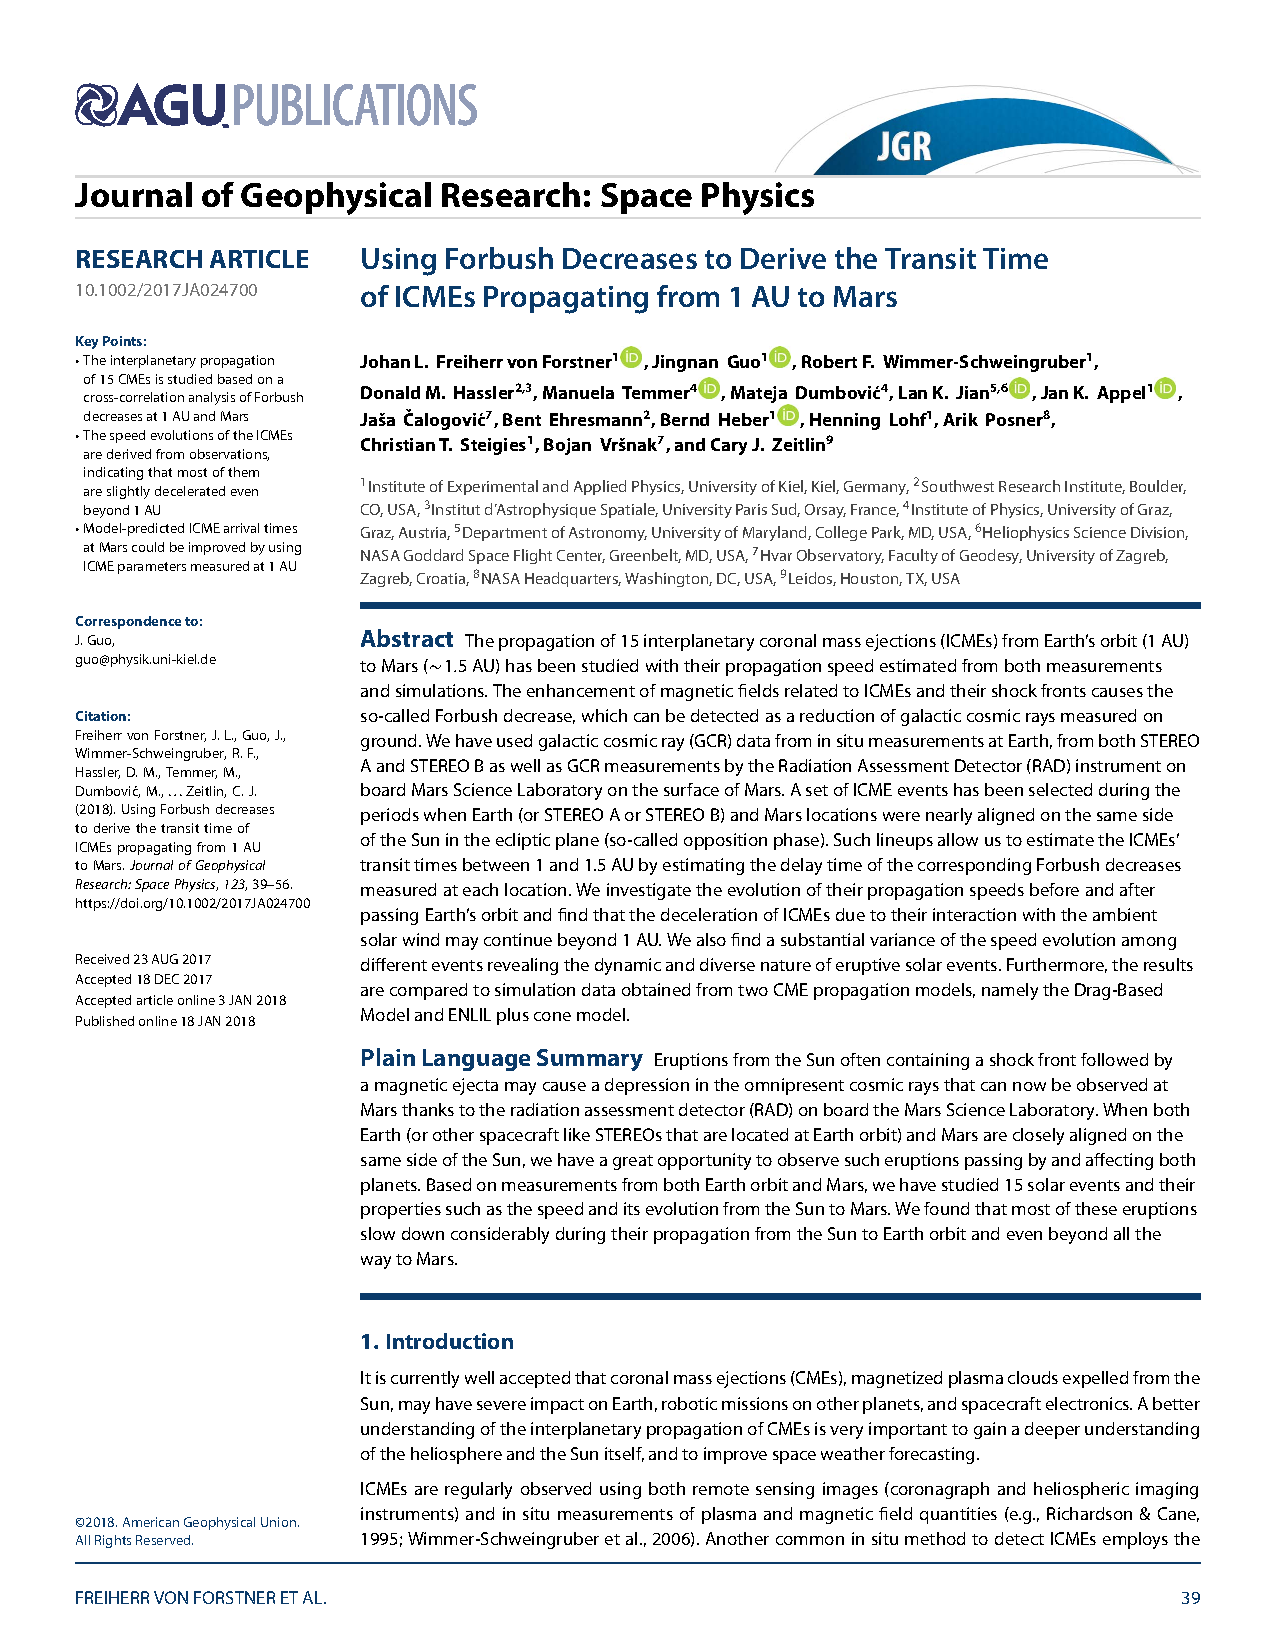
\includepdf[pages={1-2}, link, linkname=paper_forstner2018, scale=.9, pagecommand={\refstepcounter{includepdfpageJGREighteen}\label{paper_forstner2018.\theincludepdfpageJGREighteen}}]{publications/Forstner_et_al-2018-JGRSpace.pdf}
%
\addtocounter{subsubsection}{1} 
\phantomsection
\addcontentsline{toc}{subsubsection}{\arabic{chapter}.\arabic{section}.\arabic{subsection}.\arabic{subsubsection} Methods and Data}
\includepdf[pages={3-5}, link, linkname=paper_forstner2018, scale=.9, pagecommand={\refstepcounter{includepdfpageJGREighteen}\label{paper_forstner2018.\theincludepdfpageJGREighteen}}]{publications/Forstner_et_al-2018-JGRSpace.pdf}
%
\addtocounter{subsubsection}{1} 
\phantomsection
\addcontentsline{toc}{subsubsection}{\arabic{chapter}.\arabic{section}.\arabic{subsection}.\arabic{subsubsection} Results and Discussion}
\includepdf[pages={6-12}, link, linkname=paper_forstner2018, scale=.9, pagecommand={\refstepcounter{includepdfpageJGREighteen}\label{paper_forstner2018.\theincludepdfpageJGREighteen}}]{publications/Forstner_et_al-2018-JGRSpace.pdf}
%
\addtocounter{subsubsection}{1} 
\phantomsection
\addcontentsline{toc}{subsubsection}{\arabic{chapter}.\arabic{section}.\arabic{subsection}.\arabic{subsubsection} Conclusion}
\includepdf[pages={13}, link, linkname=paper_forstner2018, scale=.9, pagecommand={\refstepcounter{includepdfpageJGREighteen}\label{paper_forstner2018.\theincludepdfpageJGREighteen}}]{publications/Forstner_et_al-2018-JGRSpace.pdf}
%
\addtocounter{subsubsection}{1} 
\phantomsection
\addcontentsline{toc}{subsubsection}{\arabic{chapter}.\arabic{section}.\arabic{subsection}.\arabic{subsubsection} Appendix A: Cross-Correlation Analysis Plots for Each Event}
\includepdf[pages={14-16}, link, linkname=paper_forstner2018, scale=.9, pagecommand={\refstepcounter{includepdfpageJGREighteen}\label{paper_forstner2018.\theincludepdfpageJGREighteen}}]{publications/Forstner_et_al-2018-JGRSpace.pdf}
%
\addtocounter{subsubsection}{1} 
\phantomsection
\addcontentsline{toc}{subsubsection}{\arabic{chapter}.\arabic{section}.\arabic{subsection}.\arabic{subsubsection} References}
\includepdf[pages={17-18}, link, linkname=paper_forstner2018, scale=.9, pagecommand={\refstepcounter{includepdfpageJGREighteen}\label{paper_forstner2018.\theincludepdfpageJGREighteen}}]{publications/Forstner_et_al-2018-JGRSpace.pdf}

\chapter{Validating STEREO-HI ICME tracking using FD observations}

The following article is reproduced from \textcite{Forstner-2019} with permission from Space 
Weather, \copyright American Geophysical Union:\\

\noindent\pubcite{Forstner-2019}\\
\strut\hfill Own contribution: 90\%

\newpage
\newcounter{includepdfpageSWNineteen}

\addtocounter{subsection}{1}
\setcounter{subsubsection}{1} 
\phantomsection
\addcontentsline{toc}{subsection}{\arabic{chapter}.\arabic{section}.\arabic{subsection} Tracking and Validating ICMEs Propagating Toward Mars Using STEREO Heliospheric Imagers Combined With Forbush Decreases Detected by MSL/RAD (Publication Space Weather 2019)}
%
\phantomsection
\addcontentsline{toc}{subsubsection}{\arabic{chapter}.\arabic{section}.\arabic{subsection}.\arabic{subsubsection} Introduction}
\label{sec:paper_forstner2019}
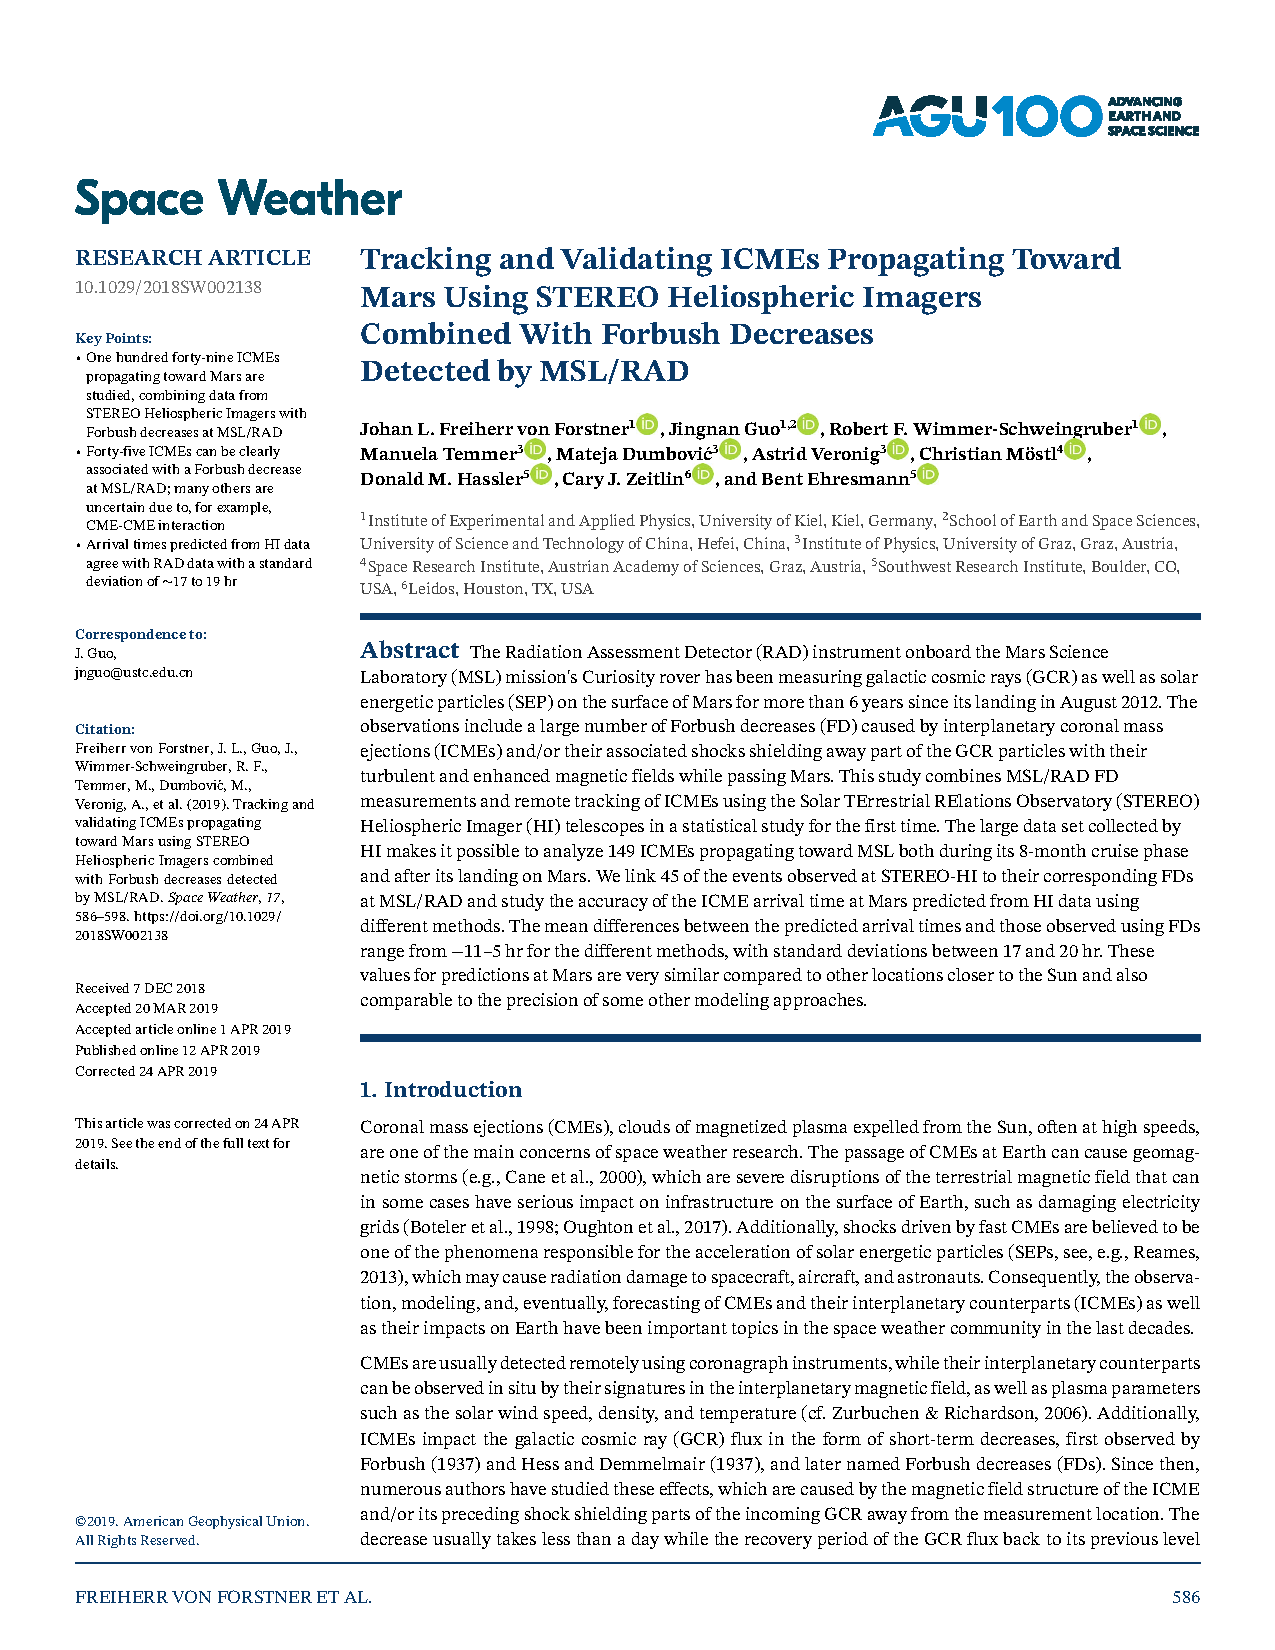
\includepdf[pages={1}, link, linkname=paper_forstner2019, scale=.95, pagecommand={\refstepcounter{includepdfpageSWNineteen}\label{paper_forstner2019.\theincludepdfpageSWNineteen}}]{publications/Forstner_et_al-2019-Space_Weather.pdf}
%
\addtocounter{subsubsection}{1} 
\phantomsection
\addcontentsline{toc}{subsubsection}{\arabic{chapter}.\arabic{section}.\arabic{subsection}.\arabic{subsubsection} Data and Methods}
\includepdf[pages={2-3}, link, linkname=paper_forstner2019, scale=.95, pagecommand={\refstepcounter{includepdfpageSWNineteen}\label{paper_forstner2019.\theincludepdfpageSWNineteen}}]{publications/Forstner_et_al-2019-Space_Weather.pdf}
%
\addtocounter{subsubsection}{1} 
\phantomsection
\addcontentsline{toc}{subsubsection}{\arabic{chapter}.\arabic{section}.\arabic{subsection}.\arabic{subsubsection} Results and Discussion}
\includepdf[pages={4-9}, link, linkname=paper_forstner2019, scale=.95, pagecommand={\refstepcounter{includepdfpageSWNineteen}\label{paper_forstner2019.\theincludepdfpageSWNineteen}}]{publications/Forstner_et_al-2019-Space_Weather.pdf}
%
\addtocounter{subsubsection}{1} 
\phantomsection
\addcontentsline{toc}{subsubsection}{\arabic{chapter}.\arabic{section}.\arabic{subsection}.\arabic{subsubsection} Conclusions and Outlook}
\includepdf[pages={10}, link, linkname=paper_forstner2019, scale=.95, pagecommand={\refstepcounter{includepdfpageSWNineteen}\label{paper_forstner2019.\theincludepdfpageSWNineteen}}]{publications/Forstner_et_al-2019-Space_Weather.pdf}
%
\addtocounter{subsubsection}{1} 
\phantomsection
\addcontentsline{toc}{subsubsection}{\arabic{chapter}.\arabic{section}.\arabic{subsection}.\arabic{subsubsection} References}
\includepdf[pages={11-13}, link, linkname=paper_forstner2019, scale=.95, pagecommand={\refstepcounter{includepdfpageSWNineteen}\label{paper_forstner2019.\theincludepdfpageSWNineteen}}]{publications/Forstner_et_al-2019-Space_Weather.pdf}

\chapter{Comparing the properties of FDs at Earth and Mars}

\TODO{Summary of the publication}

\newpage

The following article is reproduced from \textcite{Forstner-2020} from Journal of Geophysical Research: Space Physics, \copyright American Geophysical Union, under the Creative Commons CC-BY license: \ccLogo\ccAttribution\\

\pubcite{Forstner-2020}
\hfill Own contribution: 80\%

\newpage
\newcounter{includepdfpageJGRTwenty}

\addtocounter{section}{1}
\setcounter{subsection}{1} 
\phantomsection
\addcontentsline{toc}{section}{\arabic{chapter}.\arabic{section} Comparing the Properties of ICME-Induced Forbush Decreases at Earth and Mars (Publication JGR--Space Physics 2020)}
%
\phantomsection
\addcontentsline{toc}{subsection}{\arabic{chapter}.\arabic{section}.\arabic{subsection} Introduction}
\label{sec:paper_forstner2020}
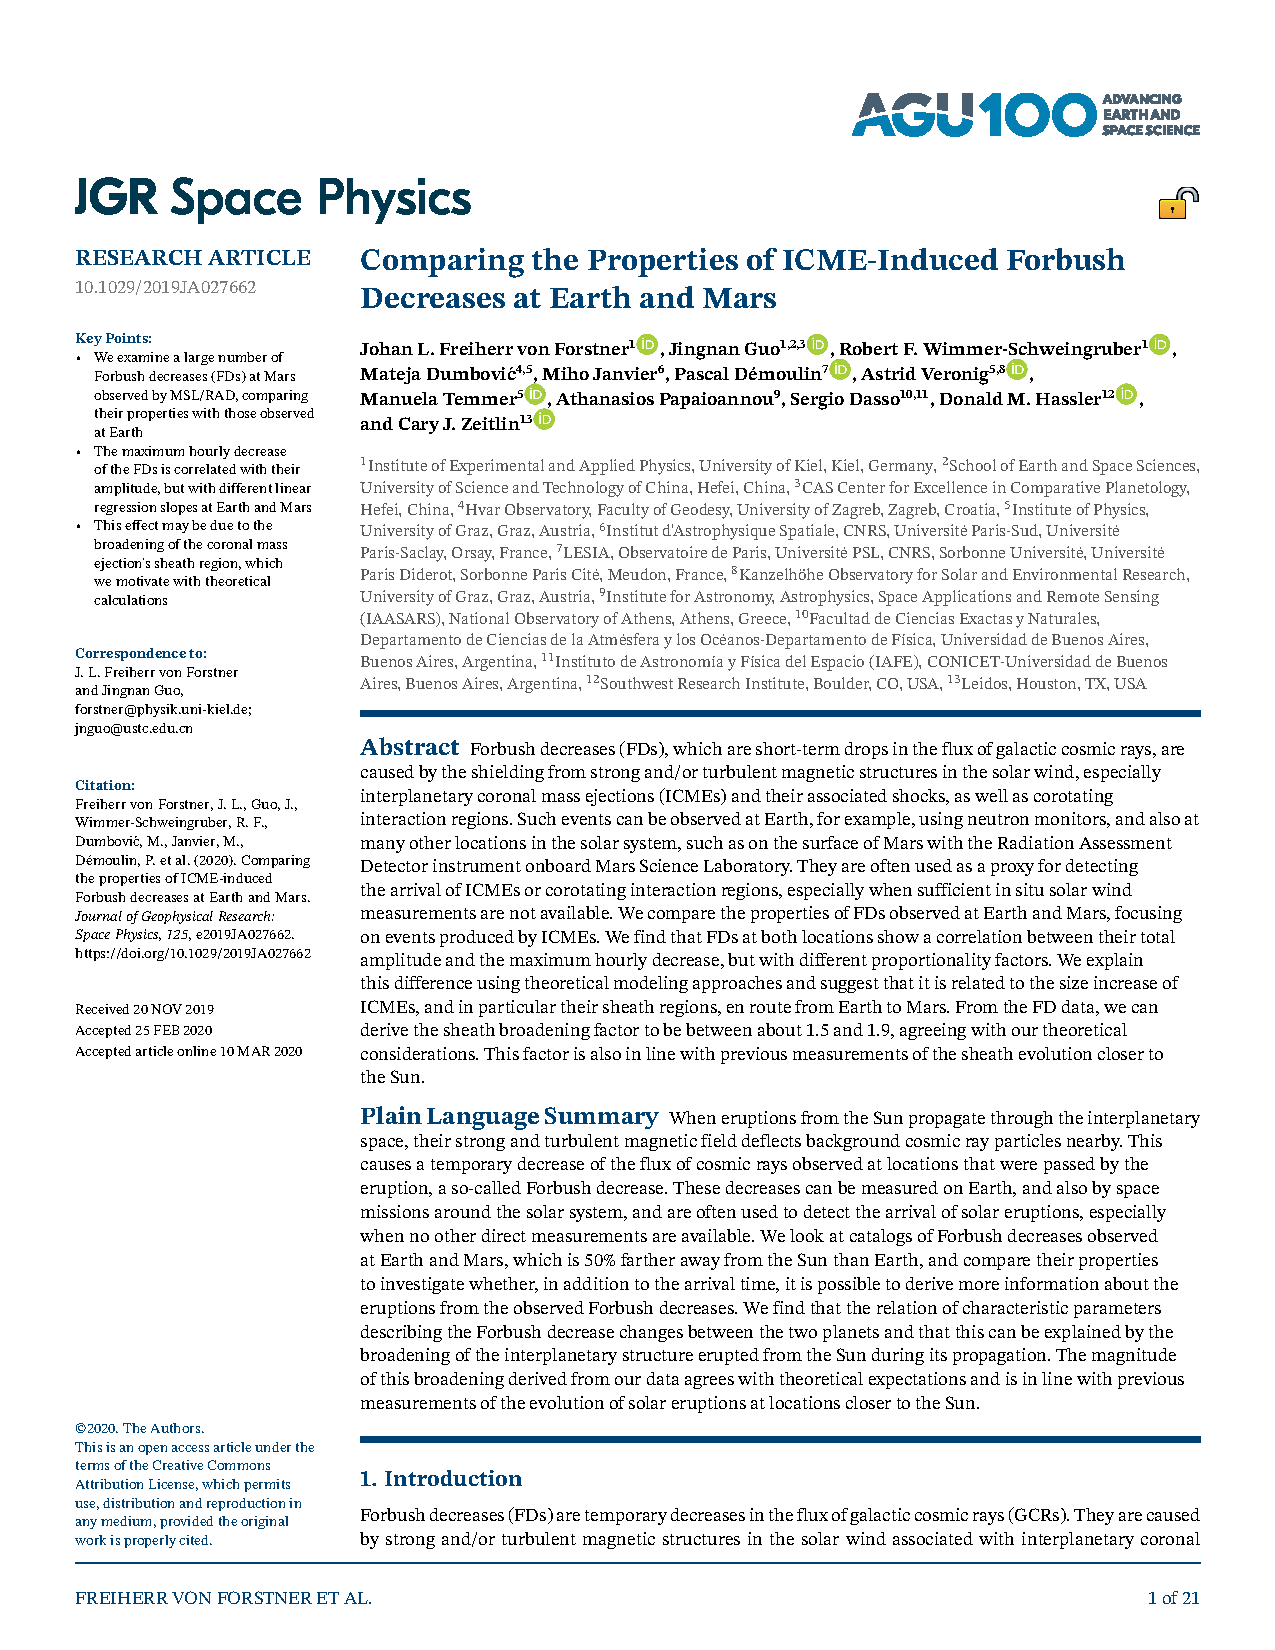
\includepdf[pages={1}, link, linkname=paper_forstner2020, scale=.95, pagecommand={\refstepcounter{includepdfpageJGRTwenty}\label{paper_forstner2020.\theincludepdfpageJGRTwenty}}]{publications/Forstner_et_al-2020-JGRSpace.pdf}
%
\addtocounter{subsection}{1} 
\phantomsection
\addcontentsline{toc}{subsection}{\arabic{chapter}.\arabic{section}.\arabic{subsection} Data Sources and Catalogs}
\includepdf[pages={2-5}, link, linkname=paper_forstner2020, scale=.95, pagecommand={\refstepcounter{includepdfpageJGRTwenty}\label{paper_forstner2020.\theincludepdfpageJGRTwenty}}]{publications/Forstner_et_al-2020-JGRSpace.pdf}
%
\addtocounter{subsection}{1} 
\phantomsection
\addcontentsline{toc}{subsection}{\arabic{chapter}.\arabic{section}.\arabic{subsection} Definitions and Methodology}
\includepdf[pages={6-7}, link, linkname=paper_forstner2020, scale=.95, pagecommand={\refstepcounter{includepdfpageJGRTwenty}\label{paper_forstner2020.\theincludepdfpageJGRTwenty}}]{publications/Forstner_et_al-2020-JGRSpace.pdf}
%
\addtocounter{subsection}{1} 
\phantomsection
\addcontentsline{toc}{subsection}{\arabic{chapter}.\arabic{section}.\arabic{subsection} Results and Discussions}
\includepdf[pages={8-16}, link, linkname=paper_forstner2020, scale=.95, pagecommand={\refstepcounter{includepdfpageJGRTwenty}\label{paper_forstner2020.\theincludepdfpageJGRTwenty}}]{publications/Forstner_et_al-2020-JGRSpace.pdf}
%
\addtocounter{subsection}{1} 
\phantomsection
\addcontentsline{toc}{subsection}{\arabic{chapter}.\arabic{section}.\arabic{subsection} Conclusions and Outlook}
%
\addtocounter{subsection}{1} 
\phantomsection
\addcontentsline{toc}{subsection}{\arabic{chapter}.\arabic{section}.\arabic{subsection} Appendix A: Location of $m_{\text{max}}$ Within the ICME Substructures}
\includepdf[pages={17-18}, link, linkname=paper_forstner2020, scale=.95, pagecommand={\refstepcounter{includepdfpageJGRTwenty}\label{paper_forstner2020.\theincludepdfpageJGRTwenty}}]{publications/Forstner_et_al-2020-JGRSpace.pdf}
%
\addtocounter{subsection}{1} 
\phantomsection
\addcontentsline{toc}{subsection}{\arabic{chapter}.\arabic{section}.\arabic{subsection} References}
\includepdf[pages={19-21}, link, linkname=paper_forstner2020, scale=.95, pagecommand={\refstepcounter{includepdfpageJGRTwenty}\label{paper_forstner2020.\theincludepdfpageJGRTwenty}}]{publications/Forstner_et_al-2020-JGRSpace.pdf}

% ********************************************************************
% Backmatter
%*******************************************************
\newpage
\markboth{}{\thepage}
\cleardoublepage
\phantomsection
\addcontentsline{toc}{chapter}{Bibliography}

\printbibliography

\cleardoublepage
%*******************************************************
% Acknowledgements
%*******************************************************
\refstepcounter{dummy}
\pdfbookmark[0]{Acknowledgements}{Acknowledgements}
\chapter*{Acknowledgements}

At this point, I want to express my gratitude to everyone who has played an important role during the course of my Ph.D. Their assistance, guidance, and support have been invaluable over the past five years. Without their help, I would not be where I am now.

First of all, I would like to thank my supervisor, Prof. Robert F. Wimmer-Schweingruber, for giving me the opportunity to join the group and work on the exciting projects - Chang'E-4/LND and SolO/EPD. He supported me in publishing these results in scientific journals and presenting them at multiple international conferences. I enjoyed discussing scientific topics with him. Those discussions inspired me and made me more productive.

I am also grateful to Prof. Jingnan Guo, who recommended me to Robert five years ago. She guided and helped me a lot on the LND projects. I hope I can have opportunities to continue our collaborations in the future. Besides, I would like to thank Prof. Dressing Nina, who provided valuable instructions and comments on the SEP paper of LND. She kindly wrote me a strong reference letter for me for the postdoc application of Caltech. That recommendation must be one of the key factors that help me to be selected from multiple candidates.

Furthermore, many thanks are given to my lovely colleagues working on LND and SOLO projects and in the Kiel group. Firstly, I would like to thank my officemate Dr. Lars Berger, for his patience and kindness every time I asked him basic and stupid questions. These discussions with him were one of the best moments that I enjoyed most. Despite that, I would like to show special thanks to him for his encouragement during finishing my thesis in the last two months. By the way, I still can not enjoy your heavy metal music. 
Secondly, I would like to show my appreciation to Dr. Verena Heidrich-Meisner, Dr. Patrick K\"{u}hl, and Dr. Marquardt Johannes for their proofreading of this thesis. They provided valuable suggestions and vastly improved the thesis.
Next, I want to express my appreciation to my colleagues in the Kiel group for their help. They are the future Ph.D., Alexander Kollhoff, Chaoran Gu, Salman Khaksarighiri, Kr\"{o}hnke Henning, as well as Dr. Daniel Pacheco, Dr. Liu Yang, Dr. Johan von Forstner, Dr. Jia Yu, and Henning Lohf.

I also want to thank my friends in Kiel, Jinru He, Lei Shao, Xuenan Li, and Xiuming Sun, who have always supported me, taken care of me, and helped me survive the tough COVID times. I remember the time that we enjoyed the fried chicken wings and played Catan all night until the following day. Thanks to those tough times, they made me stronger and more confident.

In the end, I would like to thank my parents - Aifang Wang and Fazhen Xu - for their understanding and support during my studies. 
Specifically, I would like to express my deepest love and gratitude to my wife, Zhenlin Zhu. She always has my back, and I am so lucky to have her in my life.


Further acknowledgments to the online tools for thesis writing and proofreading, including but not limited to Chatgpt, Grammarly, NotionAI, and DeepL. They are mighty in correcting grammar mistakes.
 

% At this point, I would like to thank everyone who supported me during the course of my Ph.D. studies and my work on MSL/RAD, Chang'E 4 LND, as well as Solar Orbiter EPD.

% First of all, I am grateful to my supervisor, Prof. Robert Wimmer-Schweingruber for the opportunity to work on these exciting projects, and his helpful advice. He also made it possible that these results could be published in scientific journals and presented at many international conferences. Sincere thanks also to Prof. Jingnan Guo, who supported my work since my bachelor's thesis, and who I wish all the best for her new position in China.

% Furthermore, thanks to all my colleagues in the three mission teams for their continued support and helpful discussions, including Zigong Xu, Alexander Kollhoff, and my officemate Christoph Terasa for the productive and enjoyable collaboration, e.g. on low- and high-level software for the Solar Orbiter mission, which will hopefully facilitate the EPD data analysis in the Kiel team for years to come, and to the rest of the Extraterrestrial Physics group at Kiel University. I also thank the group of Manuela Temmer and Astrid Veronig at the University of Graz and Mateja Dumbović at Hvar Observatory with whom I worked in close collaboration for many of the Forbush decrease studies, and who I enjoyed meeting regularly at the conferences in Vienna, Hvar and San Francisco.

% I additionally want to thank the bachelor and master students who supported my work during their Hiwi positions, Charlotte Büschel and Niklas Lundt, and three secondary school students, Joana Wanger, Lukas Abegg and Markus Arndt, who contributed to the data sets used in my studies during their internships in the ET group.

% I would like to thank Anne Fischer as well as Hanna Giese and Knud Schröter for their very thorough proofreading of this thesis and valuable suggestions, and my parents Kristina and Michael and my brother Julius for their moral support. 

% Last but not least, the data analysis presented in this thesis, the typesetting of the thesis itself and the generation of most of the figures were made possible by a number of open source software projects, including, but not limited to, the ones acknowledged below:

% \begin{refsection}[software.bib]
%   \nocite{*}
%   \newrefcontext[sorting=none]
%   \printbibliography[heading=none]
% \end{refsection}

\cleardoublepage
%*******************************************************
% Declaration
%*******************************************************
\refstepcounter{dummy}
\pdfbookmark[0]{Eidesstattliche Erkl\"arung}{Eidesstattliche Erkl\"arung}
\chapter*{Eidesstattliche Erkl\"arung gemäss §9 der Promotionsordnung}
%\thispagestyle{empty}
\begin{otherlanguage}{ngerman}
Ich versichere an Eides statt, dass die vorliegende Abhandlung -- abgesehen von der Beratung durch meinen Betreuer und 
der angegebenen Literatur -- nach Inhalt und Form meine eigene Arbeit ist.

Ich versichere, dass die Arbeit weder ganz noch zum Teil schon einer anderen Stelle im Rahmen eines Prüfungsverfahrens vorgelegen hat.
%
Teile dieser Arbeit wurden bereits in Fachzeitschriften veröffentlicht und sind als solche gekennzeichnet.
%
Die Quellennachweise der jeweiligen Veröffentlichungen befinden sich ausschließlich in den zugehörigen 
Literaturverzeichnissen und werden nicht im Literaturverzeichnis dieser Abhandlung aufgeführt.

Ich versichere, dass die Arbeit unter Einhaltung der Regeln guter wissenschaftlicher Praxis der 
Deutschen Forschungsgemeinschaft entstanden ist.

Ich versichere, dass von mir noch kein frühererer Promotionsversuch unternommen wurde und mir auch kein akademischer 
Grad entzogen wurde.
\end{otherlanguage}


\bigskip
 
\noindent\textit{\myLocation, \myTime}

\smallskip

\begin{flushright}
    \begin{tabular}{m{8cm}}
        \\ \hline
        \centering\myName \\
    \end{tabular}
\end{flushright}


\end{document}
